\begin{figure}[h]
\centering
\tikzset{every picture/.style={line width=0.75pt}} %set default line width to 0.75pt        
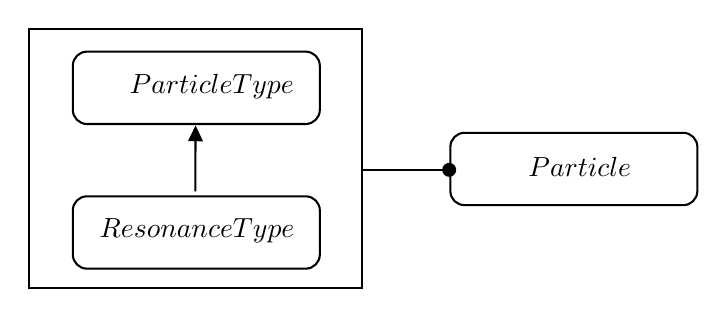
\begin{tikzpicture}[x=0.75pt,y=0.75pt,yscale=-0.85,xscale=0.85]
%uncomment if require: \path (0,300); %set diagram left start at 0, and has height of 300
%Rounded Rect [id:dp20615820737265156] 
\draw   (116.5,151) .. controls (116.5,146.58) and (120.08,143) .. (124.5,143) -- (248.5,143) .. controls (252.92,143) and (256.5,146.58) .. (256.5,151) -- (256.5,176) .. controls (256.5,180.42) and (252.92,184) .. (248.5,184) -- (124.5,184) .. controls (120.08,184) and (116.5,180.42) .. (116.5,176) -- cycle ;
%Shape: Rectangle [id:dp4661821073560425] 
\draw   (91.5,48) -- (280.5,48) -- (280.5,195) -- (91.5,195) -- cycle ;
%Rounded Rect [id:dp15238098637275865] 
\draw   (116.5,69) .. controls (116.5,64.58) and (120.08,61) .. (124.5,61) -- (248.5,61) .. controls (252.92,61) and (256.5,64.58) .. (256.5,69) -- (256.5,94) .. controls (256.5,98.42) and (252.92,102) .. (248.5,102) -- (124.5,102) .. controls (120.08,102) and (116.5,98.42) .. (116.5,94) -- cycle ;
%Rounded Rect [id:dp40566555480564326] 
\draw   (330.5,115) .. controls (330.5,110.58) and (334.08,107) .. (338.5,107) -- (462.5,107) .. controls (466.92,107) and (470.5,110.58) .. (470.5,115) -- (470.5,140) .. controls (470.5,144.42) and (466.92,148) .. (462.5,148) -- (338.5,148) .. controls (334.08,148) and (330.5,144.42) .. (330.5,140) -- cycle ;
%Straight Lines [id:da542247619427663] 
\draw    (185.93,140.15) -- (186.06,105.85) ;
\draw [shift={(186.07,102.85)}, rotate = 450.22] [fill={rgb, 255:red, 0; green, 0; blue, 0 }  ][line width=0.08]  [draw opacity=0] (8.93,-4.29) -- (0,0) -- (8.93,4.29) -- cycle    ;
%Straight Lines [id:da009375194794216335] 
\draw    (280.84,128) -- (329.84,128) ;
\draw [shift={(329.84,128)}, rotate = 0] [color={rgb, 255:red, 0; green, 0; blue, 0 }  ][fill={rgb, 255:red, 0; green, 0; blue, 0 }  ][line width=0.75]      (0, 0) circle [x radius= 3.35, y radius= 3.35]   ;

% Text Node
\draw (130,154) node [anchor=north west][inner sep=0.75pt]   [align=center] {$ResonanceType$};
% Text Node
\draw (147,72) node [anchor=north west][inner sep=0.75pt]   [align=center] {$ParticleType$};
% Text Node
\draw (373,119) node [anchor=north west][inner sep=0.75pt]   [align=center] {$Particle$};

\end{tikzpicture}
\caption{Schema della struttura del codice, come si può vedere la classe Particle non erdita proprietà dalle altre due ma usa il meccanismo della composizione.}
\end{figure}